\begin{surferPage}[无次曲面(15个尖点)]{带有15个尖点的五次曲面}
这个5次曲面具有15个$A_2$型奇异点(称为尖点)。2005年奥利弗莱布斯在一篇文章中给出了此5次曲面以及相关的一系列曲面。15个尖点中的5个看起来会跟其他10个不同。实际上这5个尖点是$A_2^{++}$型,
而另外10个尖点是$A_2^{+-}$型的(更多信息参见本图册里面的简单奇异点):
     \vspace*{-0.3em}
    \begin{center}
      \begin{tabular}{c@{\qquad}c}
        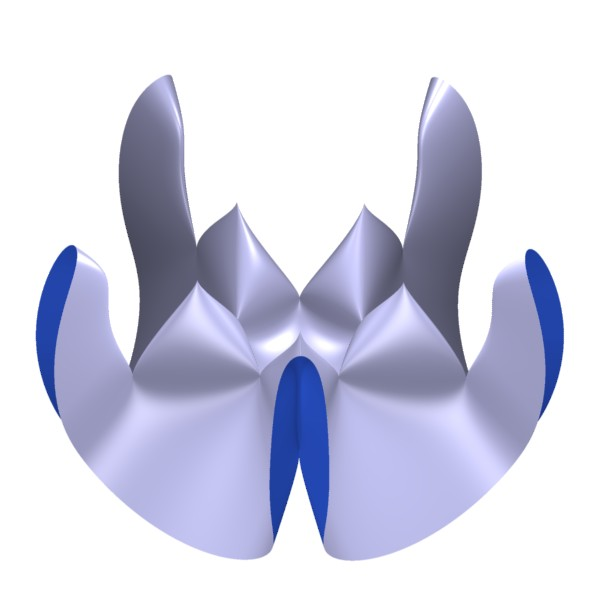
\includegraphics[height=1.2cm]{./../../common/images/dessins_quint_15a2}
        &
        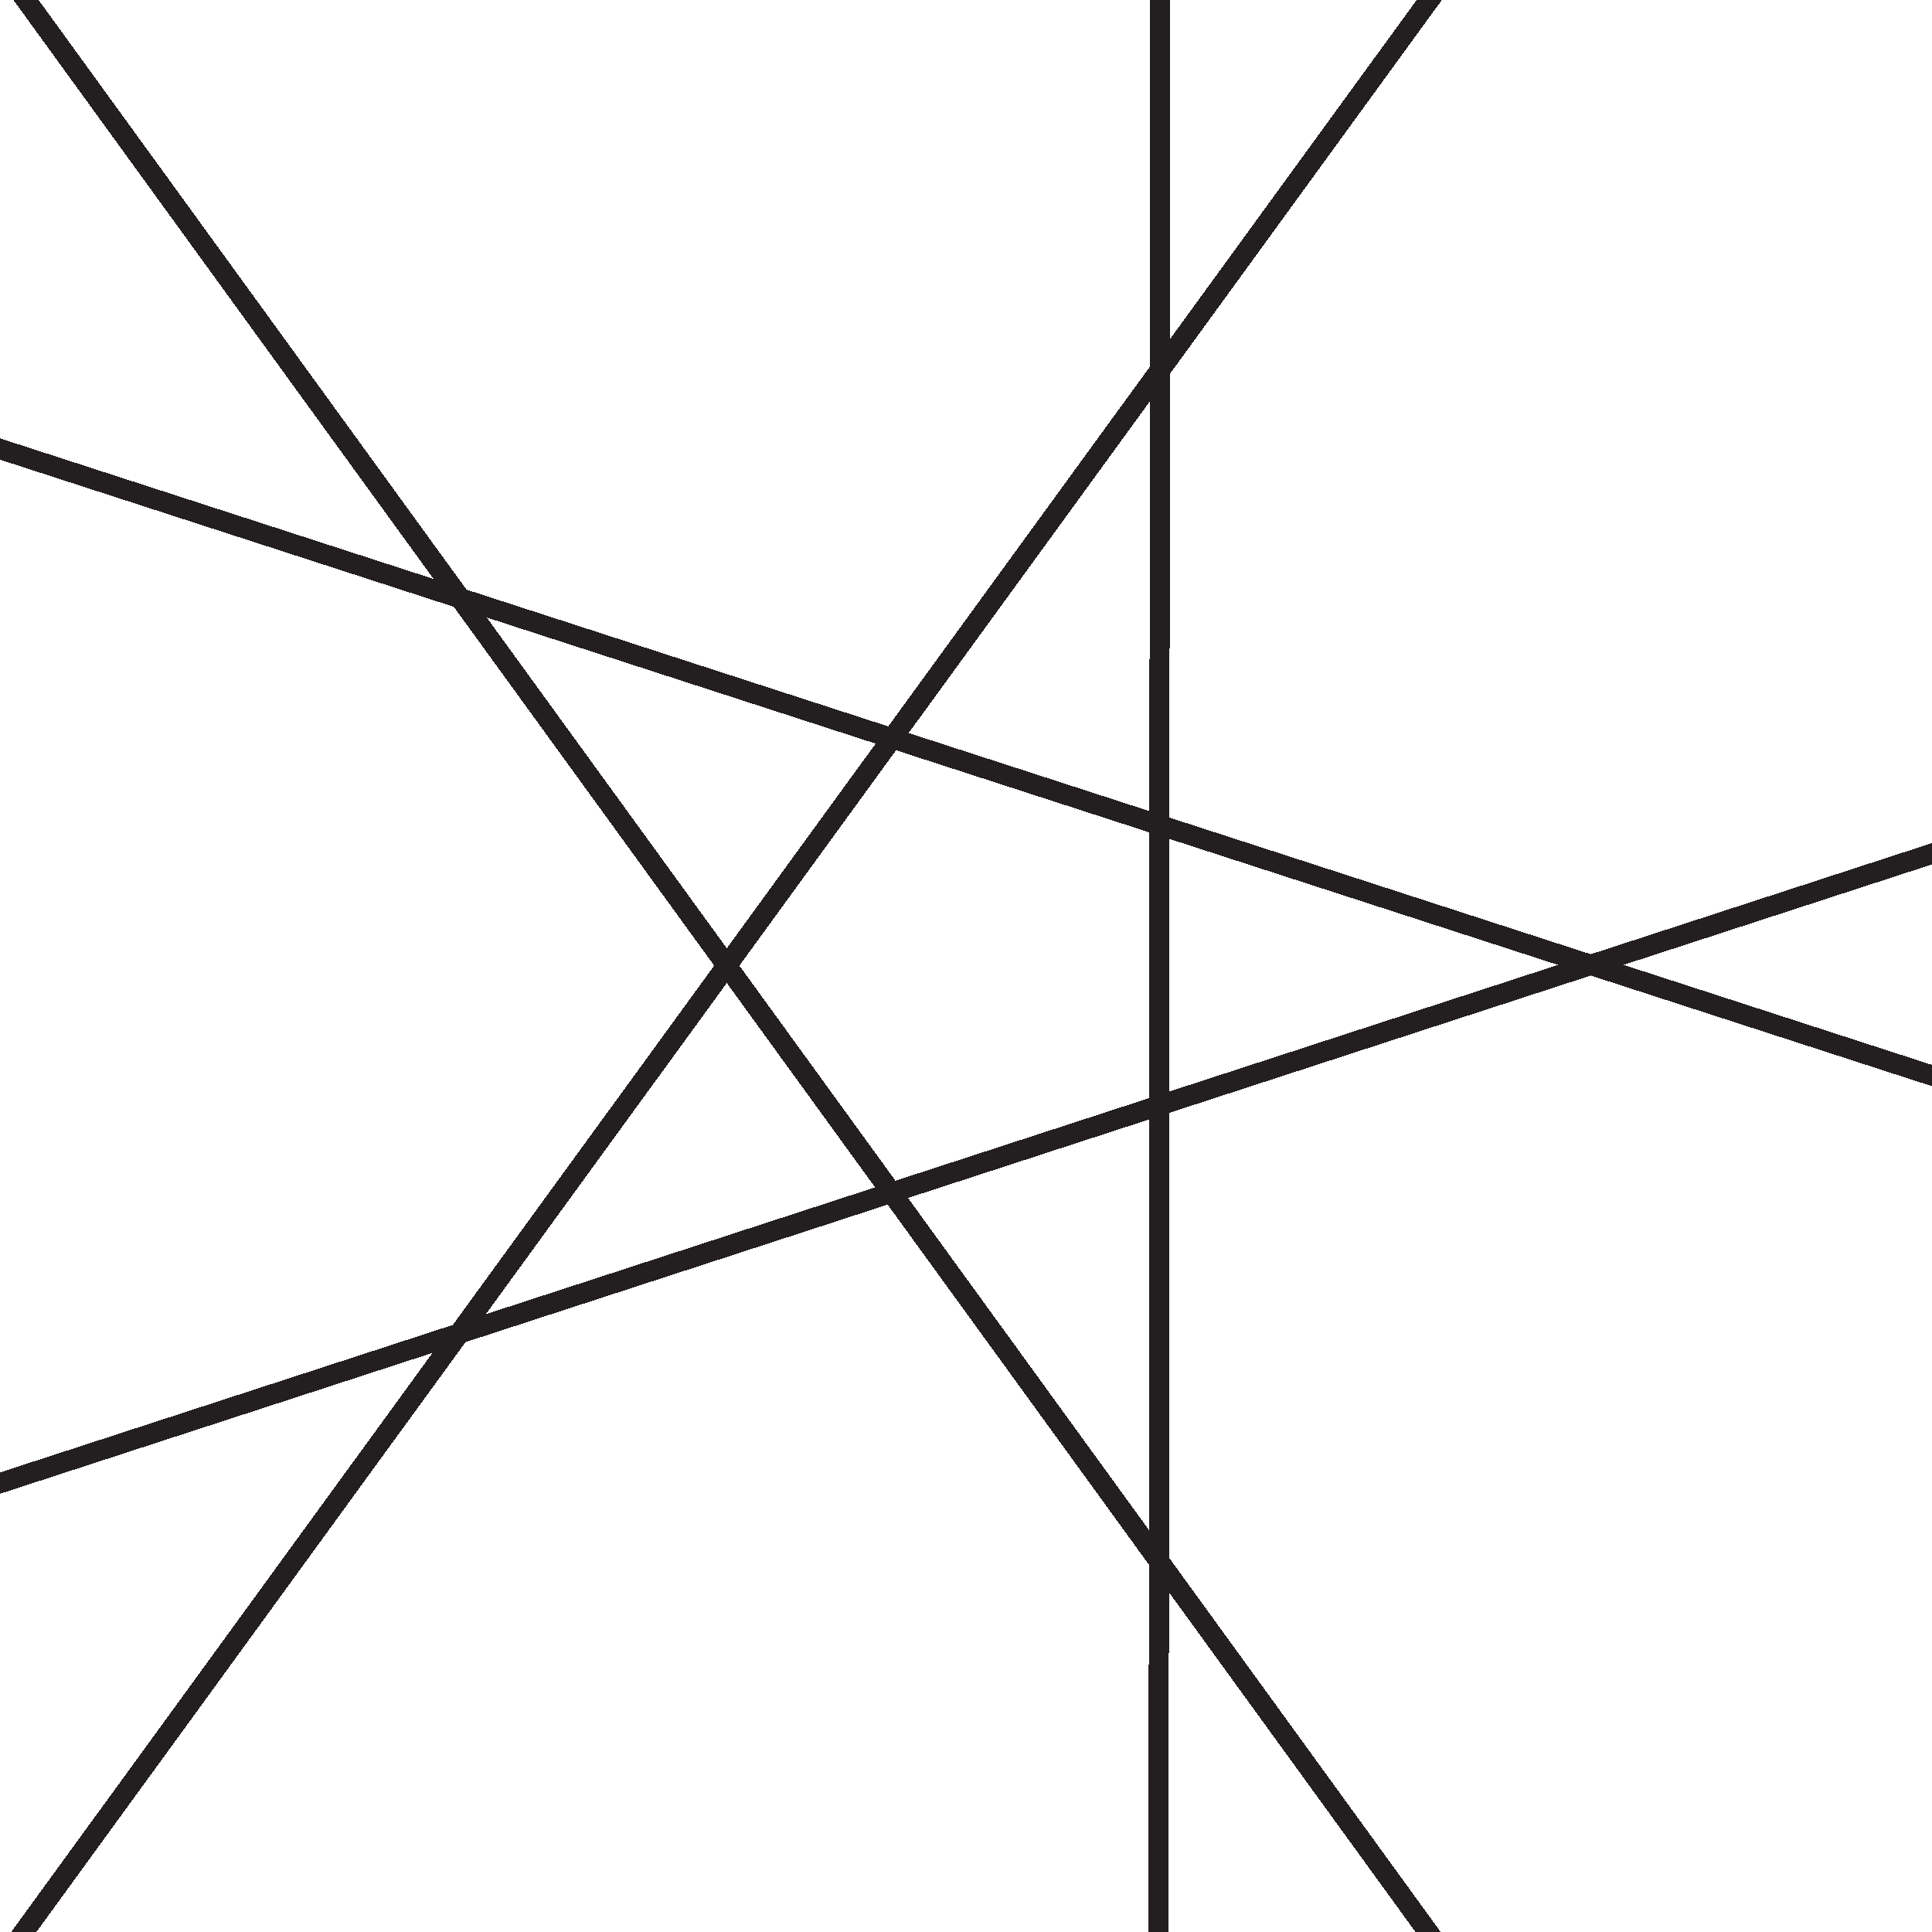
\includegraphics[height=1.2cm]{./../../common/images/rp5.pdf}
      \end{tabular}
    \end{center}
    \vspace*{-0.3em}

此曲面具有方程$S_5(x,y) + t(z)=0,$其中$S_5(x,y)$为正五边形(右图),$t(z)$是我们曾多次提起的Tchebychev多项式的一种变形。
另外一种5次曲面(左图)由沃尔夫巴斯构造出来。从中间图可以看出,它和克勒布施立方体(右图)相关。
    \vspace*{-0.3em}
    \begin{center}
      \begin{tabular}{c@{\quad}c@{\quad}c}
        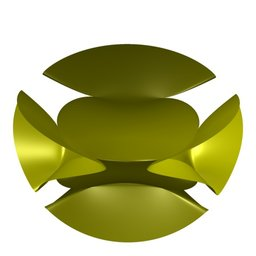
\includegraphics[height=1.2cm]{./../../common/images/barthquintic_green}
        &
        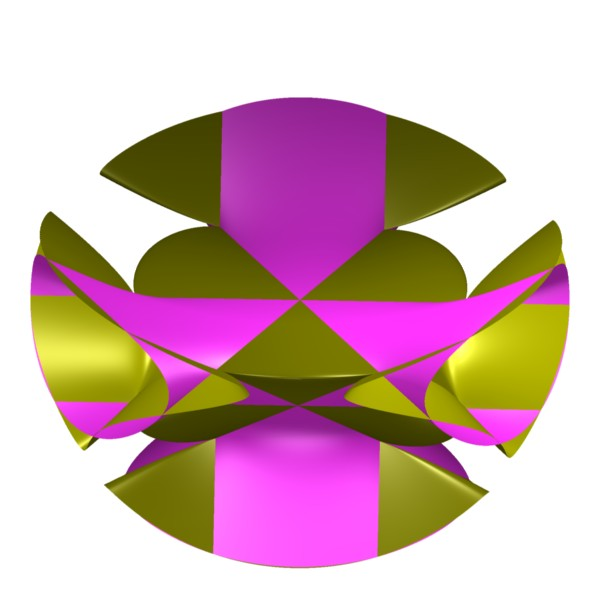
\includegraphics[height=1.2cm]{./../../common/images/barthquintic_clebschcubic}
        &
        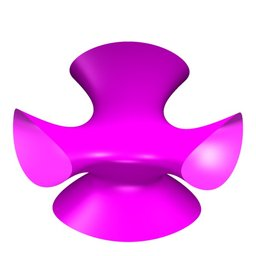
\includegraphics[height=1.2cm]{./../../common/images/clebschcubic_pink}
      \end{tabular}
    \end{center}
    \vspace*{-0.3em}
\end{surferPage}
